\documentclass[crop,tikz]{standalone}


\begin{document}

\tikzset{every picture/.style={line width=0.75pt}} %set default line width to 0.75pt        

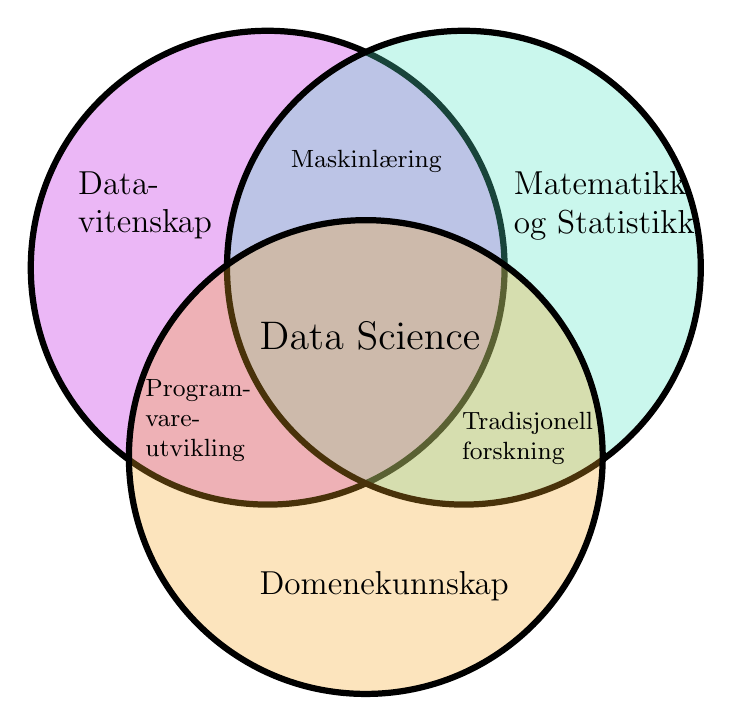
\begin{tikzpicture}[x=0.75pt,y=0.75pt,yscale=-0.5,xscale=0.5]
%uncomment if require: \path (0,672); %set diagram left start at 0, and has height of 672

%Shape: Ellipse [id:dp379509378496549] 
\draw  [fill={rgb, 255:red, 189; green, 16; blue, 224 }  ,fill opacity=0.3 ][line width=2.25]  (7,235.27) .. controls (7,109.2) and (109.2,7) .. (235.27,7) .. controls (361.34,7) and (463.54,109.2) .. (463.54,235.27) .. controls (463.54,361.34) and (361.34,463.54) .. (235.27,463.54) .. controls (109.2,463.54) and (7,361.34) .. (7,235.27) -- cycle ;
%Shape: Ellipse [id:dp47050855894352783] 
\draw  [fill={rgb, 255:red, 80; green, 227; blue, 194 }  ,fill opacity=0.3 ][line width=2.25]  (196.07,235.27) .. controls (196.07,109.2) and (298.27,7) .. (424.34,7) .. controls (550.41,7) and (652.61,109.2) .. (652.61,235.27) .. controls (652.61,361.34) and (550.41,463.54) .. (424.34,463.54) .. controls (298.27,463.54) and (196.07,361.34) .. (196.07,235.27) -- cycle ;
%Shape: Ellipse [id:dp2680287200009025] 
\draw  [fill={rgb, 255:red, 245; green, 166; blue, 35 }  ,fill opacity=0.3 ][line width=2.25]  (101.54,417.73) .. controls (101.54,291.66) and (203.74,189.46) .. (329.81,189.46) .. controls (455.88,189.46) and (558.08,291.66) .. (558.08,417.73) .. controls (558.08,543.8) and (455.88,646) .. (329.81,646) .. controls (203.74,646) and (101.54,543.8) .. (101.54,417.73) -- cycle ;

% Text Node
\draw (50,140) node [anchor=north west][inner sep=0.75pt]  [font=\large] [align=left] {Data-\\vitenskap};
% Text Node
\draw (470,140) node [anchor=north west][inner sep=0.75pt]  [font=\large] [align=left] {Matematikk \\og Statistikk};
% Text Node
\draw (225,525) node [anchor=north west][inner sep=0.75pt]  [font=\large] [align=left] {Domenekunnskap};
% Text Node
\draw (115,340) node [anchor=north west][inner sep=0.75pt]  [font=\small] [align=left] {Program-\\vare-\\utvikling};
% Text Node
\draw (420,372) node [anchor=north west][inner sep=0.75pt]  [font=\small] [align=left] {Tradisjonell \\forskning};
% Text Node
\draw (255,120) node [anchor=north west][inner sep=0.75pt]  [font=\small] [align=left] {Maskinlæring};
% Text Node
\draw (225,285) node [anchor=north west][inner sep=0.75pt]  [font=\Large] [align=left] {Data Science};

\end{tikzpicture}

\end{document}

%%% Local Variables:
%%% mode: latex
%%% TeX-master: t
%%% End:
